120. \begin{figure}[ht!]
\center{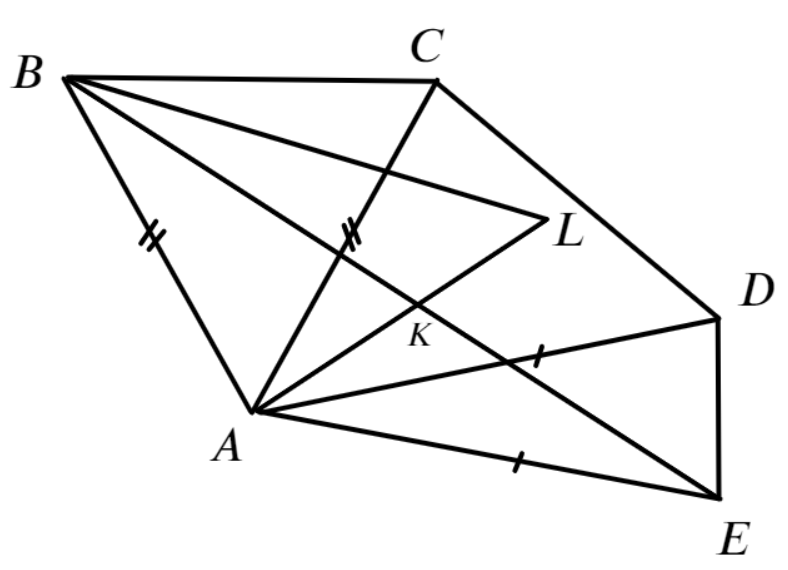
\includegraphics[scale=0.35]{g120.png}}
\end{figure}\\
Продлим медиану $AK$ на свою длину до точки $L.$ Тогда $\left.\begin{array}{l}BK=KE,\\
AK=KL,\\
\angle BKL=\angle AKE\text{ вертикальные.} \end{array}\right\}\Rightarrow \Delta AKE=\Delta BKL\text{ по I признаку}\Rightarrow
\angle ABL=\angle ABE+\angle EBL=\angle ABE+\angle BEA=\angle DAC.$ Также  $BL=AE=AD.$ Тогда
$\left.\begin{array}{l}AB=AC,\\
BL=AD,\\
\angle ABL=\angle DAC. \end{array}\right\}\Rightarrow \Delta ABL=\Delta CAD\text{ по I признаку}\Rightarrow CD=AL=2AK,$ ч.т.д.\newpage\noindent
